\documentclass[conference]{IEEEtran}
\usepackage{amsmath,amssymb,graphicx,booktabs,array,url}
\usepackage[hidelinks]{hyperref}
\usepackage{tikz}
\usetikzlibrary{arrows.meta,positioning}
\newcommand{\statusnote}[1]{\par\smallskip\noindent\textbf{Status:} #1\par\smallskip}
\newcommand{\evidencefigure}[2]{\IfFileExists{generated/#1}{\begin{figure}[!ht]\centering\includegraphics[width=\linewidth,height=.66\textheight,keepaspectratio]{generated/#1}\caption{#2}\end{figure}}{}}
\title{Image Restoration with Universal and Routed Autoencoders\\and Style-Conditioned Face-to-Sketch Generation}
\author{\IEEEauthorblockN{%%STUDENT_NAME%%}\IEEEauthorblockA{%%STUDENT_ID%%\\%%COURSE%%}}
\begin{document}
\maketitle
\begin{abstract}
This project implements four connected generative imaging workflows: a universal
denoising autoencoder, a hard-routed system of specialist autoencoders, a jointly
trained soft mixture, and a style-conditioned paired conditional GAN. The first
three share the Oxford-IIIT Pet split and corruption definitions; the fourth
uses paired FS2K photographs and sketches. The implementation uses
%%MODEL_SELECTION_PROTOCOL%% and deploys
verified ONNX inference through a React and FastAPI application started with
Docker Compose. %%ABSTRACT_STATUS%% %%ABSTRACT_FINDINGS%%
\end{abstract}
\begin{IEEEkeywords}denoising autoencoder, mixture of experts, conditional GAN, ONNX\end{IEEEkeywords}

\section{Introduction}
Image restoration reconstructs a clean target when the observed image is
affected by impulse noise, blur, or missing regions. A universal model offers a
single reconstruction path, while specialist models can allocate capacity to
individual corruption types. Hard routing introduces classifier mistakes; soft
routing permits uncertain inputs to combine several outputs. Paired sketch
generation additionally requires a style condition and an adversarial objective.
The research questions are whether specialization improves reconstruction,
how routing errors change quality, whether soft weights remain balanced, and
whether a compact conditional generator responds to the three FS2K styles.
These questions require measured results rather than assumed rankings.
The contributions are: (i) a runtime-corruption pipeline with deterministic
validation and test manifests; (ii) a compressed universal autoencoder, a
classifier-routed set of specialists, and a jointly trained soft mixture that
share one data protocol; (iii) a style-conditioned paired GAN; (iv) Optuna and
MLflow records for every task; and (v) one Docker Compose application exposing
all four workspaces through verified ONNX models.

\section{Related Research and Design Alternatives}
Autoencoders learn compact representations by forcing data through a
bottleneck \cite{hinton}, and denoising training maps corrupted inputs to clean
targets \cite{vincent}. Supervised convolutional restoration networks such as
DnCNN \cite{dncnn} and encoder-decoder networks with long skip connections such
as U-Net \cite{unet} are strong baselines. Skip connections were deliberately
not used in the restoration autoencoders: they would let the decoder copy
uncompressed input features, which the assignment's bottleneck requirement
excludes. The consequence, examined in Section~\ref{sec:discussion}, is limited
texture recovery.

SSIM evaluates local structural agreement \cite{wang}; L1 penalizes pixel
differences. Combining them provides distinct reconstruction signals, but their
weight is selected through validation. The soft system follows the mixture-of-experts
idea of Jacobs et al.\ \cite{jacobs}. Expert imbalance is a known concern
\cite{shazeer,switch}; this project uses a dense output mixture with the
assignment's batch-mean balance penalty, not the sparse routing of those works.
Conditional GANs \cite{gan,cgan} and paired translation with a U-Net generator
and local (PatchGAN) discriminator \cite{isola} motivate Task~4, using FS2K
\cite{fs2kpaper}. The compact discriminator here has a 38-pixel receptive
field; it is a local discriminator variant rather than the original 70-pixel design.

\begin{table}[!ht]\centering\caption{Alternatives investigated and the decision taken}\scriptsize
\renewcommand{\arraystretch}{1.12}\begin{tabular}{>{\raggedright\arraybackslash}p{.25\linewidth}>{\raggedright\arraybackslash}p{.36\linewidth}>{\raggedright\arraybackslash}p{.24\linewidth}}\toprule
Alternative & Evidence or reasoning & Decision\\\midrule
Restoration U-Net with long skips & Bypasses the required bottleneck \cite{unet} & Rejected\\
Dense latent vector (128 values) & Collapsed, nearly constant outputs in validation grids (objective 0.322) & Replaced by spatial latent\\
$8{\times}8$ spatial latent (512 values) & Objective 0.281; coarse shapes, large colour error & Replaced by $16{\times}16$\\
GroupNorm in the autoencoder & Per-input statistics; BatchNorm \cite{batchnorm} with tracked statistics tested next & BatchNorm adopted\\
Learning rate $10^{-3}$ & Saturated outputs in a pilot & Rejected; $\le 5{\times}10^{-4}$ searched\\
Bilinear resize + conv & Compared with PixelShuffle decoder \cite{shi} & PixelShuffle + ICNR \cite{aitken}\\
Sparse top-$k$ gating \cite{shazeer} & Only three experts; dense blend is differentiable and matches the brief & Dense softmax gate\\
Per-batch entropy regulariser \cite{switch} & Not evaluated; assignment's squared deviation kept & Squared deviation from $1/4$\\\bottomrule
\end{tabular}\end{table}
The pilot objectives in the table are the validation measurements recorded
in Section~\ref{sec:discussion} and the project's research notes; they are
exploratory sequential changes rather than controlled single-factor ablations.

\section{Data Preparation and Reproducibility}
All images are RGB and resized to $128\times128$ with bicubic interpolation.
The Oxford official trainval membership \cite{pets} is split with NumPy random seed 42,
yielding 2,944 training and 736 validation images. The official test set contains
3,669 images. The same membership is used for Tasks 1--3; breed labels do not
supervise restoration. Source archives and preparation code are retained with
manifest hashes. Test images are downloaded and resized during preparation,
but never loaded by training or hyperparameter selection.

The official FS2K annotations define 1,058 development pairs and 1,046 test
pairs \cite{fs2k}. A stratified 15\% validation split with seed 42 yields 899
training and 159 validation pairs. Training style counts are 303/298/298 and
validation counts are 54/52/53. Style labels are read from annotations, not
inferred from folder names. The official photograph-to-sketch filename mapping
is preserved. Horizontal flips are applied identically to both images in a
training pair.

\subsection{Runtime Corruptions}
Every clean training image receives a freshly sampled condition. The universal
model samples each of four conditions with equal probability; classifier and
gate batches enforce equal counts. Salt-and-pepper probability is uniform in
$[0.02,0.15]$, with selected RGB pixels set to black or white equiprobably. Blur
uses a finite separable Gaussian kernel of size 3, 5, or 7 and sigma uniform in
$[0.5,2.5]$. Occlusion samples one to three disjoint black rectangles whose
joint area approximates a sampled fraction in $[0.10,0.35]$. Disjoint horizontal
bands prevent overlap; random widths and positions vary mask geometry. This
restriction should be considered when interpreting generalization to arbitrary
real occlusions.

Validation and test manifests persist condition, seed, blur settings, and mask
coordinates. Each image has one clean condition and nine corrupted conditions.
\begin{table}[!ht]\centering\caption{Fixed validation and test severity definitions}
\begin{tabular}{lccc}\toprule Condition & Low & Medium & High\\\midrule
Salt probability & .03 & .08 & .15\\
Blur $(k,\sigma)$ & $(3,.7)$ & $(5,1.5)$ & $(7,2.5)$\\
Occlusion area & 10\% & 20\% & 35\%\\
Rectangle count & 1 & 2 & 3\\\bottomrule\end{tabular}\end{table}
Pixel rounding can slightly change the realized mask area, which is recoverable
from stored coordinates. Training corruptions are not saved as image copies.

\subsection{Evaluation Protocol and Test-Set Use}\label{sec:protocol}
All hyperparameters, architectures and checkpoints were selected using the
validation split only. The model files evaluated in this report were frozen by
SHA-256 hash before the final test run; the hashes and selected epochs are
stored in the results summary. The official test split was also evaluated for
two earlier model generations during development, so it is a held-out reporting
set rather than a set seen for the first time. Architecture, search and checkpoint
decisions used validation measurements only.

\section{Task 1: Universal Restoration}
%%AUTOENCODER_METHOD%%
No skip connection copies uncompressed features to the decoder.
\begin{equation}
\hat{x}=D(E(\tilde{x})),\quad
\mathcal{L}_{rec}=\alpha\|\hat{x}-x\|_1+(1-\alpha)(1-\mathrm{SSIM}(\hat{x},x)).
\end{equation}
SSIM uses an $11\times11$ Gaussian window with sigma 1.5, valid convolution,
$C_1=0.01^2$, and $C_2=0.03^2$. It is averaged over RGB channels and windows.
The validation objective fixes $\alpha=0.8$ for comparability across trials;
the training weight is tuned.
\begin{figure}[!ht]\centering
\begin{tikzpicture}[node distance=4mm, every node/.style={draw,rounded corners,font=\scriptsize,align=center,minimum height=7mm},>=Stealth]
\node (x) {Input\\$3\times128^2$};
\node (e) [right=of x] {Conv encoder\\%%ENCODER_FEATURES%%};
\node (z) [right=of e] {Latent\\$d$ values};
\node (d) [below=of z] {Conv decoder};
\node (y) [left=of d] {RGB reconstruction};
\draw[->] (x)--(e);\draw[->] (e)--(z);\draw[->] (z)--(d);\draw[->] (d)--(y);
\end{tikzpicture}\caption{Task 1 compressed restoration path. Tasks 2 and 3 reuse this expert architecture.}\end{figure}

\section{Task 2: Classification and Hard Routing}
A four-stage convolutional classifier uses global average pooling, dropout,
and a four-logit linear head. Multiclass cross entropy supervises the corruption
label generated by the data loader. Three independently optimized autoencoders
learn salt, blur, and occlusion restoration. A shared architecture search scores
the average validation objective across all three specialists.
\begin{equation}
r=\arg\max_k C(\tilde{x})_k,\quad
\hat{x}=\begin{cases}\tilde{x},&r=0,\\A_r(\tilde{x}),&r\ne0.\end{cases}
\end{equation}
Oracle routing selects the branch using the true manifest label; predicted
routing uses classifier argmax. Comparing these modes isolates the contribution
of routing mistakes. Clean oracle inputs have an exact identity bypass; a
misclassified clean input can be unnecessarily altered in predicted mode.
Accuracy, macro precision/recall/F1, per-class metrics, a normalized confusion
matrix, and individual routing failures are included after evaluation.

\begin{figure}[!ht]\centering
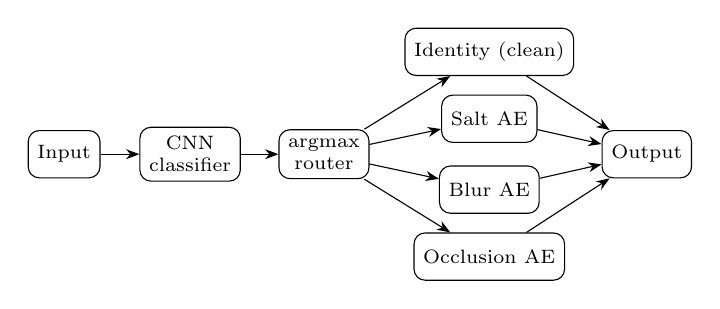
\begin{tikzpicture}[every node/.style={draw,rounded corners,font=\scriptsize,align=center,minimum height=6mm},>=Stealth]
\node (x) at (0.3,0) {Input};
\node (c) at (1.9,0) {CNN\\classifier};
\node (r) at (3.6,0) {argmax\\router};
\node (e0) at (5.7,1.3) {Identity (clean)};
\node (e1) at (5.7,0.45) {Salt AE};
\node (e2) at (5.7,-0.45) {Blur AE};
\node (e3) at (5.7,-1.3) {Occlusion AE};
\node (y) at (7.7,0) {Output};
\draw[->] (x)--(c);\draw[->] (c)--(r);
\foreach \i in {0,1,2,3} {\draw[->] (r)--(e\i);\draw[->] (e\i)--(y);}
\end{tikzpicture}\caption{Task 2 hard routing: the classifier selects exactly one branch; clean inputs bypass restoration.}\end{figure}

\section{Task 3: Joint Soft Mixture}
The gate is initialized from the trained classifier and the three experts from
Task 2. An initial two-epoch warm-up trains only the gate with experts frozen;
the experts are then unfrozen and the complete system is fine-tuned jointly.
Both stages use one Adam learning rate, searched in $[10^{-5},3\times10^{-4}]$
(selected $2.7\times10^{-4}$, below the classifier's $7.9\times10^{-4}$ and
slightly below the specialists' $3\times10^{-4}$); it is not reduced a second
time at unfreezing.
\begin{align}
w&=\mathrm{softmax}(G(\tilde{x})/\tau),\\
\hat{x}&=w_0\tilde{x}+\sum_{k=1}^{3}w_k A_k(\tilde{x}),\\
\mathcal{L}_{joint}&=\alpha\mathcal{L}_1+(1-\alpha)(1-\mathrm{SSIM})\nonumber\\
&\quad+\lambda_{cls}\mathcal{L}_{CE}+\lambda_{bal}\sum_{k=0}^{3}(\bar{w}_k-1/4)^2.
\end{align}
The balance target assumes balanced training batches. A temperature above one
softens weights; a lower value sharpens them. Mean weights per condition and
severity, distributed and dominant examples, and branches receiving under 1\%
mean weight are reported. The inference graph evaluates all branches, so it
does not inherit sparse-compute speed advantages.
\begin{figure}[!ht]\centering
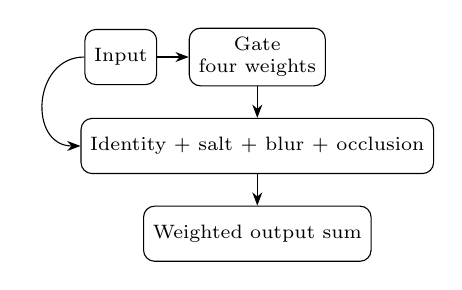
\begin{tikzpicture}[node distance=4mm, every node/.style={draw,rounded corners,font=\scriptsize,align=center,minimum height=7mm},>=Stealth]
\node (x) {Input};\node (g) [right=of x] {Gate\\four weights};
\node (b) [below=of g] {Identity + salt + blur + occlusion};
\node (s) [below=of b] {Weighted output sum};
\draw[->] (x)--(g);\draw[->] (x.west) to[out=180,in=180,looseness=1.5] (b.west);\draw[->] (g)--(b);\draw[->] (b)--(s);
\end{tikzpicture}\caption{Soft routing; hard routing instead uses argmax and executes one selected branch.}\end{figure}

\section{Task 4: Style-Conditioned Face-to-Sketch GAN}
A five-level U-Net downsamples from 128 to 4 pixels and upsamples through
skip-connected decoding stages. A learned style embedding is spatially
broadcast and concatenated with the photograph. The discriminator separately
embeds the same style, concatenating it with photograph and sketch. Its three
stride-two convolutional stages followed by a stride-one logit convolution
produce local real/fake predictions. %%GAN_METHOD%%
\begin{align}
\mathcal{L}_D&=\tfrac12[\mathrm{BCE}(D(x,y,s),1)+\mathrm{BCE}(D(x,G(x,s),s),0)],\\
\mathcal{L}_G&=\mathrm{BCE}(D(x,G(x,s),s),1)+\lambda_1\|G(x,s)-y\|_1.
\end{align}
Discriminator real/fake losses and generator adversarial/reconstruction losses
are logged separately. The same fixed validation photographs are saved every
five epochs. Only the generator is deployed. Cross-style outputs on one photo
are qualitative evidence; paired metrics apply to its annotated style only.

\begin{figure}[!ht]\centering
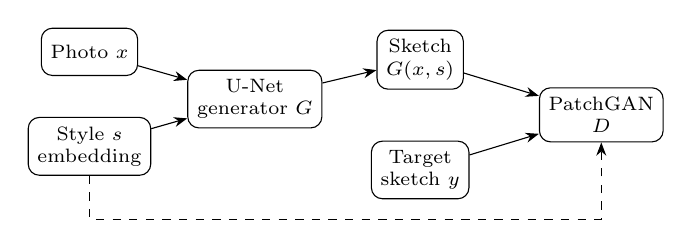
\begin{tikzpicture}[every node/.style={draw,rounded corners,font=\scriptsize,align=center,minimum height=6mm},>=Stealth]
\node (p) at (0.4,1.0) {Photo $x$};
\node (s) at (0.4,-0.2) {Style $s$\\embedding};
\node (g) at (2.5,0.4) {U-Net\\generator $G$};
\node (y) at (4.6,0.9) {Sketch\\$G(x,s)$};
\node (t) at (4.6,-0.5) {Target\\sketch $y$};
\node (d) at (6.9,0.2) {PatchGAN\\$D$};
\draw[->] (p)--(g);\draw[->] (s)--(g);\draw[->] (g)--(y);
\draw[->] (y)--(d);\draw[->] (t)--(d);
\draw[->,dashed] (s.south) -- ++(0,-0.55) -| (d.south);
\end{tikzpicture}\caption{Task 4 conditional GAN. The style embedding enters both $G$ and $D$ (dashed); $D$ outputs a map of local real/fake scores.}\end{figure}


\section{Hyperparameter Search and Training}
Optuna TPE samples configurations and median pruning stops unpromising
individual-model trials \cite{optuna,optunapaper}. Short trials use %%TRIAL_BUDGET%%; each study records its actual
budget and trial outcomes. The shared specialist study evaluates all three
specialists and does not use intermediate pruning. %%FINAL_TRAINING%% Adam \cite{adam} is used; GAN
optimizers use $(\beta_1,\beta_2)=(0.5,0.999)$. CUDA runs use mixed precision;
gradient norms are clipped to five. Checkpoints include optimizer, scaler,
random state, epoch, configuration, and data hashes for recovery.

\begin{table}[!ht]\centering\caption{Search spaces (selected model generation)}\scriptsize
\begin{tabular}{p{.25\linewidth}p{.65\linewidth}}\toprule Study & Searched parameters\\\midrule
Universal & %%UNIVERSAL_SEARCH%%\\
Classifier & LR $10^{-4}$--$.003$; batch 16/32/64; base 8/16/24; dropout 0--.3; weight decay $10^{-6}$--$10^{-3}$\\
Specialists & Shared LR, batch, base, latent, dropout, $\alpha$ as universal\\
Soft & LR $10^{-5}$--$.0003$; batch 16/32/64; $\tau$ .5--2; $\lambda_{cls}$ .02--.3; $\lambda_{bal}$ .001--.1; $\alpha$ .6--.95\\
GAN & %%GAN_SEARCH%%\\\bottomrule
\end{tabular}\end{table}
MLflow records configurations, losses, validation metrics and sample artifacts
\cite{mlflow}. %%RUNTIME_STORAGE%% Limited studies cannot support a claim of
globally optimal architectures.

\section{Evaluation and Results}
PSNR is computed per image with range one and then averaged. SSIM and L1 use
the same preprocessing for every system. Clean identity PSNR is capped at
100 dB through the numeric floor on mean-squared error. Each pet test image has
ten deterministic input conditions (36,690 inputs in a full evaluation).
Per-image CSVs preserve routing labels, errors and scores. Subset evaluations
are explicitly labelled and must not be represented as full test results.
%%RESULTS%%

\section{Discussion of Results}\label{sec:discussion}
%%DISCUSSION%%

\section{Application Architecture and Deployment}
The React/Tailwind interface provides four workspaces in one application.
FastAPI validates JPEG, PNG and WebP uploads, rejects files over 10 MB and
oversized decoded images, applies optional reproducible corruption, and runs
ONNX Runtime CPU inference. It returns input/output PNGs, route probabilities
or soft weights, and inference latency. Runtime corruption makes the clean
reference available for an error map; an arbitrary uploaded corrupted image
does not provide an assumed ground truth.
\begin{table}[!ht]\centering\caption{Backend endpoints}\scriptsize
\begin{tabular}{>{\raggedright\arraybackslash}p{.42\linewidth}>{\raggedright\arraybackslash}p{.46\linewidth}}\toprule Endpoint & Purpose\\\midrule
GET \texttt{/api/health} & Per-model and per-workspace readiness\\
GET \texttt{/api/samples} & Clean sample images\\
GET \texttt{/api/experiments} & Test metrics and MLflow run records\\
POST \texttt{/api/corrupt} & Reproducible corruption preview\\
POST \texttt{/api/universal-restoration} & Task 1 inference\\
POST \texttt{/api/hard-routing} & Task 2: probabilities, expert, output\\
POST \texttt{/api/soft-mixture} & Task 3: four weights, output\\
POST \texttt{/api/face-to-sketch} & Task 4: photo and style to sketch\\\bottomrule
\end{tabular}\end{table}

The frontend is served by Nginx and proxies API requests to the backend.
Docker Compose starts both containers using
\texttt{docker compose up --build}; the browser URL is
\url{http://localhost:8080}. Model and result directories are mounted read-only.
Session initialization is excluded from inference timing. Missing models,
synthetic test checkpoints and failed checksum verification produce a clear
unavailable-model state rather than substitute output.

ONNX export checks random, black and white inputs for batches of one and two,
including all three GAN styles. Acceptance uses absolute tolerance $10^{-4}$
and relative tolerance $10^{-3}$ for every output. Actual maximum deviations
are stored in the deployment manifest. The complete soft inference pipeline is
one graph; the classifier and specialists are separate graphs for hard routing.

\begin{figure}[!ht]\centering
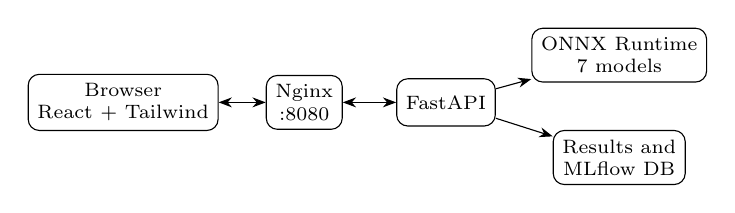
\begin{tikzpicture}[every node/.style={draw,rounded corners,font=\scriptsize,align=center,minimum height=6mm},>=Stealth]
\node (b) at (0.9,0) {Browser\\React + Tailwind};
\node (n) at (3.2,0) {Nginx\\:8080};
\node (f) at (5.0,0) {FastAPI};
\node (o) at (7.2,0.6) {ONNX Runtime\\7 models};
\node (m) at (7.2,-0.7) {Results and\\MLflow DB};
\draw[<->] (b)--(n);\draw[<->] (n)--(f);\draw[->] (f)--(o);\draw[->] (f)--(m);
\end{tikzpicture}\caption{Deployment: two Docker Compose services; model and result files are mounted read-only into the backend.}\end{figure}
%%APPLICATION_EVIDENCE%%
%%EXTERNAL_LINKS%%

\section{Limitations and Conclusion}
The main limitations are the following. (1) The compact bottleneck discards
fine texture, which appears to cap reconstruction near the level reached on clean inputs,
so blur restoration does not exceed the uncorrected input on average.
(2) Optuna searches used short trials (three epochs, 40 batches) and few trials,
so the selected configurations are the best of a small search, not a global
optimum; in three studies the best trial was the seeded starting configuration.
(3) The classifier confuses clean and low-severity blurred inputs, and the soft
gate shares that ambiguity. (4) The sketch generator produces smooth, pale
sketches without hatching; style~3 has only 46 test pairs, so its scores are
noisy. (5) Single-corruption training does not establish reliable
mixed-corruption restoration, and disjoint-band masks do not cover all real
occlusion geometries. (6) Inference is $128\times128$ on CPU; larger uploads are
resized. (7) Final training used a CPU after free GPU quota was exhausted, which
limited schedule length. (8) The soft mixture keeps its warm-up learning rate
after unfreezing the experts instead of lowering it, as the assignment suggests;
the effect of such a drop was not tested.
Future work should enlarge the latent for blur, add a sharpening or perceptual
loss, run longer GAN schedules with more Optuna trials on a GPU, and evaluate
mixed corruptions.
%%CONCLUSION_STATUS%%

\appendices
\section{AI Use and Verification}
\begin{table}[!ht]\centering\caption{AI tools used, purpose and verification}\scriptsize
\renewcommand{\arraystretch}{1.12}\begin{tabular}{>{\raggedright\arraybackslash}p{.16\linewidth}>{\raggedright\arraybackslash}p{.34\linewidth}>{\raggedright\arraybackslash}p{.32\linewidth}}\toprule
Tool & Used for & How outputs were checked\\\midrule
OpenAI Codex & Reading the assignment, finding sources, drafting models, training and evaluation code, FastAPI/React code, Colab notebook, tests, first report draft & 20 automated tests (corruptions, balanced batches, paired augmentation, SSIM, bottleneck, gradients through all mixture branches, style conditioning, upload validation, resume, ONNX), validation grids, ONNX-vs-PyTorch comparison, Docker runs\\
Anthropic Claude (Claude Code) & Final audit of the repository against the assignment, report revision (protocol, discussion, limitations), documentation and repository packaging & Numbers in the discussion are computed from the saved result files by the report script; documents compared with files; tests re-run\\
Google Stitch & Original interface design (exports retained in the repository) & Controls compared with implemented functions; decorative mock-up metrics omitted\\\bottomrule
\end{tabular}\end{table}
A soft-mixture dropout-mode mismatch found by ONNX consistency testing was
corrected. Synthetic-data tests verify mechanics only; dataset performance
comes from saved real checkpoints evaluated on deterministic manifests.
The student remains responsible for understanding and explaining every
component.

\begin{thebibliography}{99}
\bibitem{vincent} P. Vincent et al., ``Stacked denoising autoencoders: Learning useful representations in a deep network with a local denoising criterion,'' JMLR, vol. 11, pp. 3371--3408, 2010.
\bibitem{wang} Z. Wang, A. C. Bovik, H. R. Sheikh, and E. P. Simoncelli, ``Image quality assessment: From error visibility to structural similarity,'' IEEE TIP, vol. 13, no. 4, pp. 600--612, 2004.
\bibitem{shazeer} N. Shazeer et al., ``Outrageously large neural networks: The sparsely-gated mixture-of-experts layer,'' arXiv:1701.06538, 2017.
\bibitem{isola} P. Isola, J.-Y. Zhu, T. Zhou, and A. A. Efros, ``Image-to-image translation with conditional adversarial networks,'' CVPR, pp. 1125--1134, 2017.
\bibitem{pets} O. M. Parkhi et al., ``Cats and dogs,'' CVPR, 2012. Dataset: \url{https://www.robots.ox.ac.uk/~vgg/data/pets/}.
\bibitem{fs2k} FS2K dataset, official release, 2021. \url{https://github.com/DengPingFan/FS2K}.
\bibitem{optuna} Optuna documentation, efficient optimization algorithms. \url{https://optuna.readthedocs.io/en/stable/tutorial/10_key_features/003_efficient_optimization_algorithms.html}.
\bibitem{mlflow} MLflow documentation, experiment tracking. \url{https://mlflow.org/docs/latest/ml/tracking/}.
\bibitem{shi} W. Shi et al., ``Real-time single image and video super-resolution using an efficient sub-pixel convolutional neural network,'' CVPR, 2016. \url{https://arxiv.org/abs/1609.05158}.
\bibitem{aitken} A. Aitken et al., ``Checkerboard artifact free sub-pixel convolution: A note on sub-pixel convolution, resize convolution and convolution resize,'' arXiv:1707.02937, 2017.
\bibitem{hinton} G. E. Hinton and R. R. Salakhutdinov, ``Reducing the dimensionality of data with neural networks,'' Science, vol. 313, no. 5786, pp. 504--507, 2006.
\bibitem{dncnn} K. Zhang, W. Zuo, Y. Chen, D. Meng, and L. Zhang, ``Beyond a Gaussian denoiser: Residual learning of deep CNN for image denoising,'' IEEE TIP, vol. 26, no. 7, pp. 3142--3155, 2017.
\bibitem{unet} O. Ronneberger, P. Fischer, and T. Brox, ``U-Net: Convolutional networks for biomedical image segmentation,'' MICCAI, 2015.
\bibitem{jacobs} R. A. Jacobs, M. I. Jordan, S. J. Nowlan, and G. E. Hinton, ``Adaptive mixtures of local experts,'' Neural Computation, vol. 3, no. 1, pp. 79--87, 1991.
\bibitem{switch} W. Fedus, B. Zoph, and N. Shazeer, ``Switch Transformers: Scaling to trillion parameter models with simple and efficient sparsity,'' JMLR, vol. 23, no. 120, 2022.
\bibitem{gan} I. Goodfellow et al., ``Generative adversarial nets,'' NeurIPS, 2014.
\bibitem{cgan} M. Mirza and S. Osindero, ``Conditional generative adversarial nets,'' arXiv:1411.1784, 2014.
\bibitem{fs2kpaper} D.-P. Fan et al., ``Facial-sketch synthesis: A new challenge,'' Machine Intelligence Research, vol. 19, no. 4, pp. 257--287, 2022.
\bibitem{adam} D. P. Kingma and J. Ba, ``Adam: A method for stochastic optimization,'' ICLR, 2015.
\bibitem{optunapaper} T. Akiba, S. Sano, T. Yanase, T. Ohta, and M. Koyama, ``Optuna: A next-generation hyperparameter optimization framework,'' KDD, 2019.
\bibitem{batchnorm} S. Ioffe and C. Szegedy, ``Batch normalization: Accelerating deep network training by reducing internal covariate shift,'' ICML, 2015.
\end{thebibliography}
\end{document}
